\documentclass{QITthesis}


\begin{document}

\fancyhf{}
\fancyfoot[C]{\zihao{-5}\tnr\thepage}
\renewcommand{\headrulewidth}{0pt}
\pagenumbering{Roman}
\begin{abstract}
    \zihao{-4}
    \setlength{\baselineskip}{20pt}
    将Wistar大鼠随机分为5组:正常对照组、模型对照组、皂苷低剂量组、皂苷中剂量组和皂苷高剂量组。饲料中添加1\%乳清酸建立大鼠脂肪肝模型,并同时分别给予不同剂量的海参皂苷(0.01\%、0.03\%、0.05\%),连续饲喂10d。分别测定大鼠血清总胆固醇(Total cholesterol,TC)、甘油三酯(Triglyceride,TG)、高密度脂蛋白胆固醇(High density lipoprotein-cholesterol,HDL-C)含量,大鼠肝脏TC、TG、磷脂(phospholipid,PL)含量,以及肝脏中脂肪酸合成酶(FAS)的活性。结果显示海参皂苷可降低血清和肝脏脂肪含量,对脂肪肝具有很好的预防作用。

    \vspace{\baselineskip}\bfseries\heiti 关键词:
    \normalfont\heiti 海参;皂苷;脂肪肝;乳清酸;脂肪代谢
\end{abstract}

\newpage
\ctexset{abstractname=\zihao{3}\tnr\bfseries\centering Abstract\vspace{.75\baselineskip}}
\begin{abstract}
    \zihao{-4}
    \tnr
    \setlength{\baselineskip}{20pt}
    Male Wistar rats were randomly divided into five groups, including normal group, control group, low, medium and high dose saponin group. Model rats were established by with 1\% dietary orotic acid. Saponin tested group were given diets incorporated with saponin at the levels of 0.01\%, 0.03\% and 0.05\%, respectively. After 10 days feeding, Serum total cholesterol (TC), triglyceride (TG), high density lipoprotein-cholesterol (HDL-c), hepatic lipid concentrations (TG, TC and phospholipids) and the activities of hepatic fatty acid synthase (FAS) were determined. The saponin of sea cucumber could improve the serum and hepatic lipids accumulation, and is beneficial to prevent fatty liver.

    \vspace{\baselineskip}\zihao{-4}\tnr\bfseries Keywords:
    \zihao{-4}\tnr\normalfont sea cucumber; saponin; fatty liver; orotic acid; lipid bolism
\end{abstract}

\ctexset{
    section={
      numbering=false,
      format=\zihao{3}\heiti\centering,
      beforeskip=.7\baselineskip,
      afterskip=.7\baselineskip,
      fixskip=true,
      break=\newpage
     }
}

\tableofcontents

\ctexset{
    section={
      numbering=true,
      number=\arabic{section},
      format=\raggedright\zihao{3},
      numberformat=\tnr,
      titleformat=\heiti,
      aftername=\ ,
      beforeskip=.7\baselineskip,
      afterskip=.7\baselineskip,
      fixskip=true,
      break=\newpage
     }
}

\section{前言}
\zihao{-4}
\setlength{\baselineskip}{20pt}
\fancyhf{}
\renewcommand{\headrulewidth}{0.5pt}
\fancyhead[C]{\zihao{-5}毕业论文(设计)题目}
\fancyfoot[C]{\zihao{-5}\tnr\thepage}
\pagenumbering{arabic}
\subsection{海参的简介}
\subsubsection{海参的定义}

海参(Holothurian,sea cucumber)属于无脊椎动物、棘皮动物门、海参纲。广义的海参包括海参纲所有的种类。水产上的海参系指那些可供食用的干海参。别名又叫刺参,海瓜,海鼠。世界各大洋均有海参分布,栖息于温带或亚热带波静水稳、海藻茂密的岩礁海域。
海参的再生力很强,受到刺激或处于不良环境下,如水质污浊,氧气缺乏,身体常强力收缩,压迫内脏从肛门排出,这种现象称为排脏现象。内脏排出后能再生新的内脏。少数海参被横切为2--3段,各段也能再生为完整个体。

\subsubsection{海参的特征}

1.外形特征

体呈圆筒状,长10--20厘米,特大的可达30厘米,色暗,多肉刺。触手轮形,17--30个,一般为20个。触手坛囊发达。海参繁衍在地球上比原始鱼类更早,大概在六亿多年前的前寒武纪就开始存在,是现存最早的生物物种,有海洋活化石之称。经历几次地球大毁灭都得以生存下来,数度见证地球的变迁。口在前端,多偏于腹面。内骨骼退化为微小骨片。

\begin{figure}[H]
    \centering
    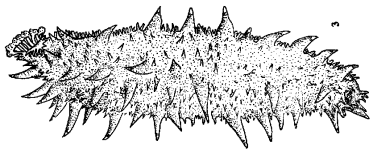
\includegraphics[width=.5\textwidth]{example_figures/图片1.png}
    \caption{刺参形态}
\end{figure}

2.生物特征

(1)变色

海参能随着居处环境而变化体色。生活在岩礁附近的海参,为棕色或深褐色;而居住在在海藻、海草中的海参则为绿色。海参的这种体色变化,可以有效的躲过天敌的伤害。

(2)休眠

\dots\dots\dots

\subsection{海参的生物活性物质}
\subsubsection{海参皂苷}

糖链中单糖的组成、位置及数量决定了皂苷分子结构的多样性,按照苷元的类型将海参皂苷分为两种,海参烷型(holostane)苷元一般18(20)-内酯环,非海参烷型(nonholostane)苷元有18(16)-内酯环或无内酯环结构。在其构效关系的研究中,其苷元上18(20)-内酯基团和靠近该基团的氧基对于保持皂苷的各种生物活性有重要意义。糖链中单糖组成有D-木糖、奎诺糖、D-葡萄糖、D-3-O-甲基葡萄糖、D-3-O-甲基木糖。

\begin{figure}[H]
    \centering
    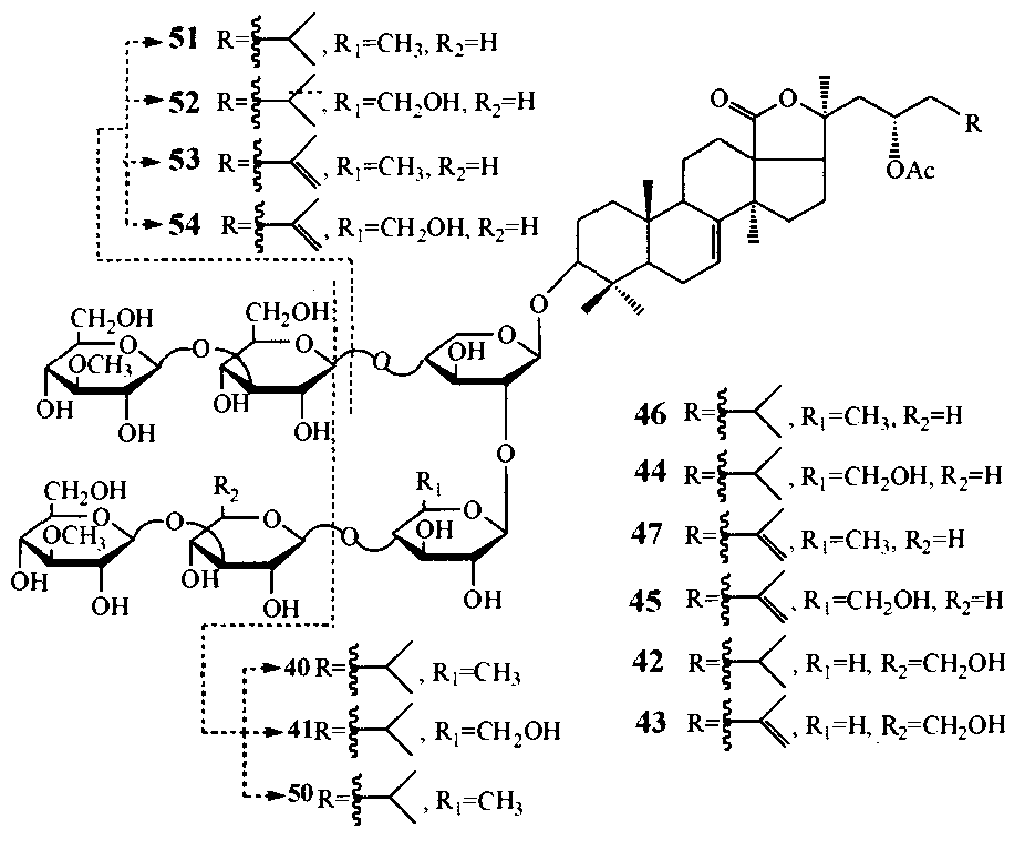
\includegraphics[width=.5\textwidth]{example_figures/图片2.png}
    \caption{刺参中海参皂苷的化学结构}
\end{figure}

\subsubsection{海参胶原蛋白}

海参胶原蛋白的类型尚不清楚,但是其氨基酸组成与人的I型胶原蛋白更接近。海参体壁是海参主要的食用或药用部位,主要构成为上皮组织和真皮结缔组织,海参真皮组织的细胞间充填着胶原等纤维成分和蛋白聚糖,以及糖蛋白等无定型间质,即细胞外基质(ECM)\footnote{细胞外基质(ECM),是由动物细胞合成并分泌到胞外、分布在细胞表面或细胞之间的大分子,主要是一些多糖和蛋白,或蛋白聚糖。}。经加工后的海参胶原蛋白的高甘氨酸含量与羟脯氨酸、羟赖氨酸的存在,表明海参蛋白以胶原蛋白为主体。

\section{实验方法}
\subsection{动物分组与饲料配比}

大鼠饲育室内适应3d后,随机分成5组:正常对照组、模型对照组、皂苷低剂量组、皂苷中剂量组、皂苷高剂量组,每组7只。饲料中添加1\%乳清酸,诱导成脂肪肝模型。各组饲料配比如表\ref{tab:t1}所示:

\begin{table}[H]
    \zihao{5}
    \centering
    \caption{动物饲料配比}
    \label{tab:t1}
    \begin{tabular}{ccccc}
        \toprule
                     & 基础饲料(g/kg) & 玉米油(g/kg) & 乳清酸(g/kg) & 皂苷(g/kg) \\
        \midrule
        正常对照组   & 980            & 20           & /            & /          \\
        模型对照组   & 970            & 20           & 10           & /          \\
        皂苷低剂量组 & 969.9          & 20           & 10           & 0.1        \\
        \bottomrule
    \end{tabular}
\end{table}

\section{计算公式}
\subsection{计算公式及其标注范例}

为了使负载电流连续且脉动小,通常串接L值较大的电感,即使电路工作在CCM模式下,当电路工作于稳态时,负载电压的平均值为:

\begin{equation}
    U_{\mathrm{o}}=\frac{t_{\mathrm{on}}}{t_{\mathrm{on}}+t_{\mathrm{off}}} E=\frac{t_{\mathrm{on}}}{T} E=u E
    \label{eq:e1}
\end{equation}

式\eqref{eq:e1}说明了XX之间的关系。

\section{结论与展望}

本章是毕业论文的总结,是整篇论文的归宿,应精炼、准确、完整。应着重阐述自己的创造性成果及其在本研究领域中的意义、作用,还可进一步提出需要讨论的问题和建议。

\subsection{主要结论}

\dots\dots\dots

\subsection{研究展望}

\dots\dots\dots

\ctexset{
    section={
      numbering=false,
      format=\zihao{3}\heiti\centering,
      beforeskip=.7\baselineskip,
      afterskip=.7\baselineskip,
      fixskip=true,
      break=\newpage
     }
}

\nocite{*}
\printbibliography
\addcontentsline{toc}{section}{参考文献}

\section{致\hspace{.5\ccwd}谢}

致谢对象主要是指导教师、在学术方面对完成毕业论文(设计)有直接贡献与较重要帮助的团体和人士。不得书写与论文工作无关的人和事。致谢词应谦虚诚恳,内容简洁明了,实事求是,切忌浮夸和庸俗之词。字数不得超过本页。例如:

大学学习生涯即将结束,回首过去的四年历程,心里感慨万千。\dots\dots。在论文即将结束之际,特向所有关心和帮助过我的老师、同学、同事、朋友和亲人们致以诚挚的谢意。
首先,衷心感谢\dots\dots。

其次,要感谢\dots\dots。

再次,在论文研究期间,我得到了\dots\dots 帮助,\dots\dots 在此我向他们表示衷心的感谢。

最后,我要感谢\dots\dots,正是他们的爱不断地激励和鼓舞我前进。

\appendix
\setcounter{figure}{0}
\setcounter{table}{0}
\setcounter{equation}{0}

\section{}

1.论文的附录依次为附录A、附录B、附录C等编号。如果只有一个附录,也应编为“附录A”。

2.附录中的图、表、公式的命名方法也采用正文提到的图、表、公式命名方法,只不过将章的序号换成附录的序号。附如“图A-5 ×××”代表附录A的第5个图。其他依次类推。

3.附录作为主体部分的补充,并不是必须的。

下列内容可以作为附录编于论文后。

(1)为了整篇论文材料的完整,但编入正文又有损于编排的条理性和逻辑性,这一材料包括比正文更为详尽的信息、研究方法和技术更深入的叙述,对了解正文内容有用的补充信息等;

(2)由于篇幅过大或取材于复制品而不便于编入正文的材料;

(3)不便于编入正文的罕见珍贵资料;

(4)对一般读者并非必要阅读,但对本专业同行有参考价值的资料;

(5)某些重要原始数据、数学推导、计算程序、框图、结构图、注释、统计表、计算机打印输出件等。

\end{document}